% Full chain: pdflatex -> bibtex -> pdflatex -> pdflatex
\documentclass[11pt,en]{elegantpaper}
\usepackage{float}
\title{Ensembling learning applied to ACLR:\\ Artificial Characters Learning Problem}
\author{Wangzhihui Mei 2019124044 6603385}
\institute{CCNU-UOW JI}

% \version{0.09}
\date{}

% cmd for this doc
\usepackage{array}
\newcommand{\ccr}[1]{\makecell{{\color{#1}\rule{1cm}{1cm}}}}

\begin{document}

\maketitle

% \begin{abstract}
% This documentation illustrates the usage of the \href{https://github.com/ElegantLaTeX/ElegantPaper}{ElegantPaper} template. This template is based on the standard \LaTeX{} article class, which is designed for working paper writing. With this template, you can get rid of all the worries about the format and merely focus on writing. For any question, please leave a message on \href{https://github.com/ElegantLaTeX/ElegantPaper/issues}{GitHub::ElegantPaper/issues}. Want to know more about Elegant\LaTeX{} Templates? Please visit: \href{https://github.com/ElegantLaTeX}{https://github.com/ElegantLaTeX}.\par
% \keywords{Elegant\LaTeX{}, Working Paper, Template}
% \end{abstract}


\section{Introduction}
This database has been artificially generated by using a first order theory which describes the structure of ten capital letters of the English alphabet and a random choice theorem prover which accounts for etherogeneity in the instances. The capital letters represented are the following: A, C, D, E, F, G, H, L, P, R. Each instance is structured and is described by a set of segments (lines) which resemble the way an automatic program would segment an image. 

Each instance is stored in a separate file whose format is the following:
\begin{lstlisting}
CLASS OBJNUM TYPE XX1 YY1 XX2 YY2 SIZE   DIAG
1     0      line 0   0   0   13  13.00  45.28
1     1      line 20  0   22  15  15.13  45.28
1     2      line 0   13  22  15  22.09  45.28
1     3      line 0   13  0   27  14.00  45.28
1     4      line 22  15  23  39  24.02  45.28
1     5      line 0   27  23  39  25.94  45.28
\end{lstlisting}

\begin{figure}[h]
	\centering
	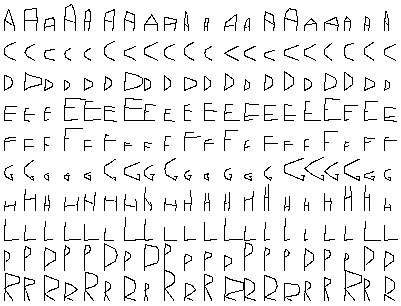
\includegraphics[width=0.5\textwidth]{image/chars}
	\caption{The generated characters}
	\label{chars}
\end{figure}

where CLASS is an integer number indicating the class as described below, OBJNUM is an integer identifier of a segment (starting from 0) in the instance and the remaining columns represent attribute values. \cite{schapire1999improved}.

The generated character image is like Figure \ref{chars}


\section{Model construction and parameter optimization}
\subsection{Data pre-process}
The character described by segments is represented as the vertex pair, we transform them to binary grid ($12\times 8$), like Figure \ref{transform}.

\begin{figure}[h]
	\centering
	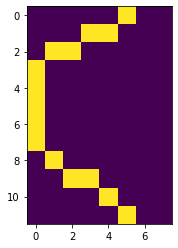
\includegraphics[width=0.3\textwidth]{image/C_array}
	\caption{The representation of "C"}
	\label{transform}
\end{figure}

Then the problem is transformed into one like the MNIST classification problem. The feature is the flattened 0-1 pixel, whose dimension is $96\times 1$, the label is "A", "C", "D", "E", "F", 
"G", "H", "L", "P", "R", which correspond to the numbers 0 through 9. 


We got 6000 training data from the primitive dataset. We shuffled them and use 70\% of the data as training data, 30\% as test data. The label distribution of training data is like Figure \ref{dist_y}
\begin{figure}[h]
	\centering
	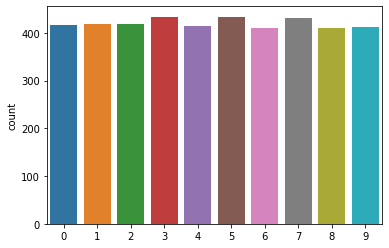
\includegraphics[width=0.4\textwidth]{image/dis_y}
	\caption{The label distribution of training data}
	\label{dist_y}
\end{figure}

\subsection{Model construction}
I applied linear models(Linear Regression, SGD, SVM), bayes model, neural network model(MLP), decision tree model, random forest model, extra tree model, and them ensemble them as voting model.
\subsubsection{Logistic Regression Model}
Regarding logistic regression, it can be summarized in one sentence: Logistic regression assumes that the data obey Bernoulli distribution, and uses the gradient likelihood method to solve the parameters through the maximum likelihood function method to achieve the purpose of classifying the data.

Our parameter tuning:
\begin{itemize}
	\item multi\_class: In this case, the pattern only belong to one class, we set it to 'multinomial'
	\item max\_iter: Set the maximum number of iterations taken for the solvers to converge to 1000.
	\item solver: For multiclass problems, only ‘newton-cg’, ‘sag’, ‘saga’ and ‘lbfgs’ handle multinomial loss; ‘liblinear’ is limited to one-versus-rest schemes, we tried and selected 'saga'.
	\item n\_jobs: Set to -1 to use all CPU cores to calculation.
	\item penalty: Set to 'l1' to get better weight sparsity.
\end{itemize}

\subsubsection{SGD}
This model is Linear classifiers with SGD training. Stochastic gradient descent(SGD) uses only one sample at a time to calculate the gradient of the objective function. The formula is:
$$\theta=\theta-\alpha \nabla_{\theta} J\left(\theta ; x^{i}, j^{i}\right)$$
The cost function is:
\begin{equation}
	J{train}(\theta)=\frac{1}{m}\sum{i=1}^{m}\frac{1}{2}(h_{\theta}(x^{(i)})-y^{(i)})^{2} = \frac{1}{m}\sum{i=1}^{m}cost(\theta;x^i,j^i)
\end{equation}
Where $\operatorname{cost}\left(\theta ; x^{i}, j^{i}\right)=\frac{1}{2}\left(h_{\theta}\left(x^{(i)}\right)-y^{(i)}\right)^{2}$

Use the loss function of each sample to derive the partial gradient of $\theta$ to get the corresponding gradient to update $\theta$:
$$\theta_{j} = \theta_{j} + \alpha(y^i - h_{\theta}(x^i))x{j}^{i}$$

Stochastic gradient descent is iteratively updated once by each sample, the calculation is very fast and suitable for updating the model online. However, the problem with SGD is that there is more noise than BGD, so that SGD does not go to the overall optimization direction every iteration, and the search process in the solution space seems blind. 

When using SGD we can choose to start with a learning rate of 1.0 or 0.1. Check it on the verification set at intervals.If the cost does not drop, the learning rate is halved.

Our parameter tuning:
\begin{itemize}
	\item loss: Set to ‘log’ loss to give logistic regression, a probabilistic classifier. 
	\item penalty: Set to 'l2'
	\item n\_job: Set to -1 to use all processors.
	\item learning\_rate: ‘optimal’: $eta = 1.0 / (alpha * (t + t0))$ where $t0$ is chosen by a heuristic proposed by Leon Bottou\cite{bottou2003stochastic}.
\end{itemize}

\subsubsection{SVM}
We applied grid search to find the optimized $C$ and $gamma$. We applied binary search method and  narrow the search iteratively. The we got the optimized $C=4.5$ and $gamma=0.06$, see in Figure \ref{bestsvm}.

\begin{figure}[h]
	\centering
	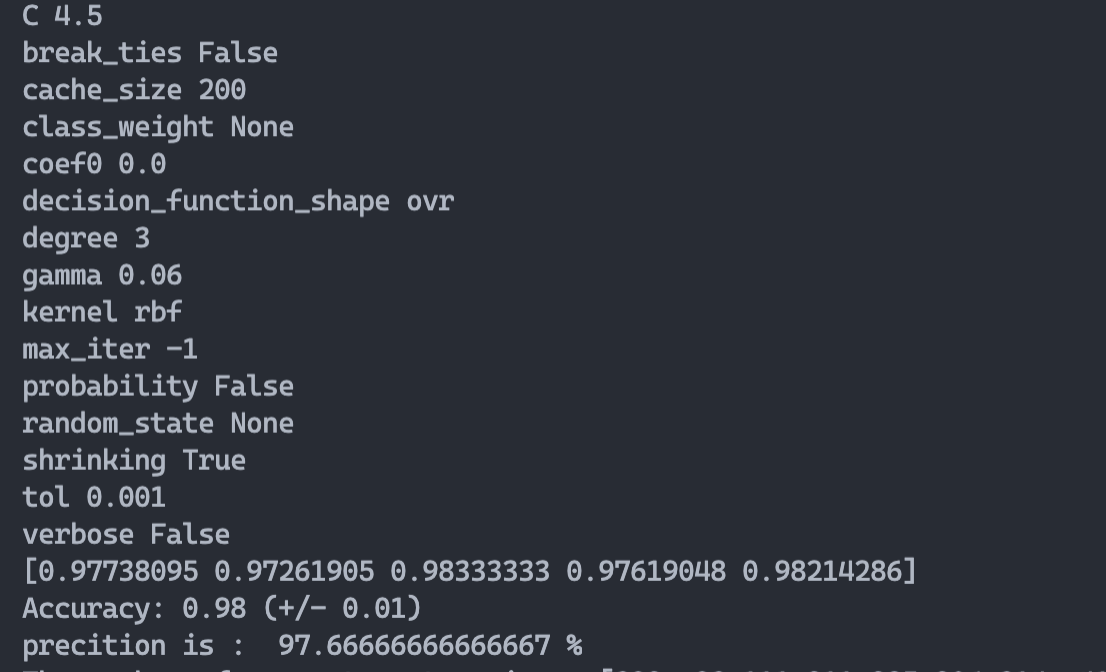
\includegraphics[width=.5\textwidth]{image/bestsvm}
	\caption{Grid search SVM parameters}
	\label{bestsvm}
\end{figure}


My parameter tuning:
\begin{itemize}
	\item C: Regularization parameter. The strength of the regularization is inversely proportional to C. Must be strictly positive. 
	\item kernel: 'rbf'
	\item gamma: 0.06, Kernel coefficient for ‘rbf’, ‘poly’ and ‘sigmoid’.


\end{itemize}


This is the number of support vectors of each class accordingly: [389  90 109 207 285 203 308  44 236 199].
\subsubsection{Decision Tree}
Decision tree is a machine learning method using statistical probability analysis. It represents a kind of mapping between object attributes and object values, and each one in the tree represents a judgment condition indicating an object attribute, which corresponds to an object that meets the condition. The leaves of the tree represent the prediction results of the object.

We use grid search to find the best parameters, see in Figure \ref{bestdt}.
\begin{figure}[h]
	\centering
	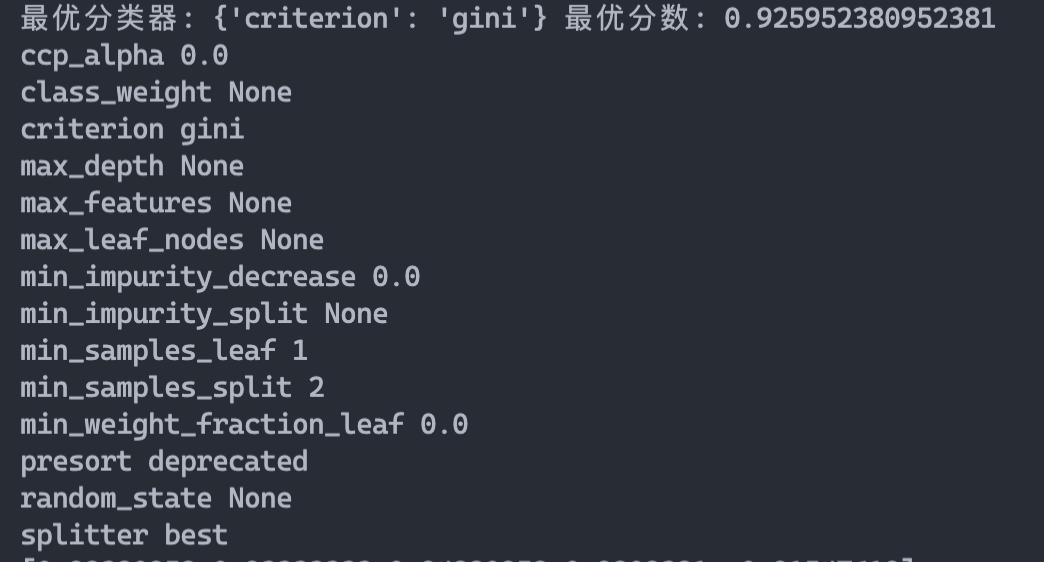
\includegraphics[width=.5\textwidth]{image/bestdt}
	\caption{Grid search decision tree parameters}
	\label{bestdt}
\end{figure}

My parameter tuning:
\begin{itemize}
	\item criterion: 'gini'. Supported criteria are “gini” for the Gini impurity.
	\item min\_samples\_leaf: 1. The minimum number of samples required to be at a leaf node. 
	\item min\_samples\_split: 2. The minimum number of samples required to split an internal node.
\end{itemize}


\subsubsection{Random Forest}
Random forest is to build a forest in a random way. There are many decision trees in the forest. There is no relationship between each decision tree in the random forest. After getting the forest, when a new input sample enters, let each decision tree in the forest make a judgment to see which category this sample should belong to, and then see which category is selected the most , Predict which category this sample is.

The main focus parameter is n\_estimators. Generally, the larger the n\_estimator, the better the model performs, but n\_estimator is too large, the boundary revenue is little, i.e., the model convergence is met. We tried 10,50,100,1000, the n\_estimator setting to 100 can perform well enough and realize the balance of the performance-calculation trade-off.

My parameter tuning:
\begin{itemize}
	\item n\_estimators: 100. The number of trees in the forest.
	\item oob\_score: True. The score outside the bag reflects the generalization ability of a model after fitting. 
	\item criterion: gini. The function to measure the quality of a split
\end{itemize}

\subsubsection{Extratree}
ET or Extra-Trees (Extremely Randomized Trees) were proposed by Pierre Geurts et. al. in 2006\cite{geurts2006kernelizing}. This algorithm is very similar to the random forest algorithm, and is composed of many decision trees. But there are two main differences between this algorithm and random forest:

1. The random forest uses the Bagging model, and ET uses all training samples to obtain each decision tree, that is, each decision tree applies the same all training samples;

2. Random forest obtains the best bifurcation attribute in a random subset, and ET obtains the bifurcation value completely randomly, so as to bifurcate the decision tree.

The tuning process is similar to Random Forest:
\begin{itemize}
	\item n\_estimators: 100. The number of trees in the forest.
	\item oob\_score: True. Whether to use out-of-bag samples to estimate the generalization accuracy.
	\item criterion: gini. The function to measure the quality of a split
\end{itemize}

\subsubsection{MLP}
We use a 4-layer MLP as classifier, with the hidden layer of 96-node and 192-node.

We applied some tricks to it: Integer multiple number of hidden layer may perform better.

Parameter tuning:
\begin{itemize}
	\item solver='sgd', 
    \item activation='relu',
    \item learning\_rate\_init=.1,
\end{itemize}

\subsection{Model Ensembling}
Ensemble modeling is a process where multiple diverse models are created to predict an outcome, either by using many different modeling algorithms or using different training data sets. The ensemble model then aggregates the prediction of each base model and results in once final prediction for the unseen data. The motivation for using ensemble models is to reduce the generalization error of the prediction. As long as the base models are diverse and independent, the prediction error of the model decreases when the ensemble approach is used. The approach seeks the wisdom of crowds in making a prediction. Even though the ensemble model has multiple base models within the model, it acts and performs as a single model. Most of the practical data mining solutions utilize ensemble modeling techniques. Chapter 4 Classification covers the approaches of different ensemble modeling techniques and their implementation in detail.

In this task, I applied Voting method. Voting is a combination strategy for classification problems in integrated learning. The basic idea is to select the most output class among all machine learning algorithms.

There are two types of output of classification machine learning algorithms: one is to directly output class labels, and the other is to output class probabilities. Using the former to vote is called hard voting (majority / hard voting), and using it to classify is called soft voting ( Soft voting). VotingClassifier in sklearn is the implementation of voting method.


\subsubsection{Hard mode}
The final result is determined by the minority obeying the majority; I applied all classifiers above to ensemble to one VotingClassifier. The structure is like Figure \ref{vcl}
\begin{figure}[h]
	\centering
	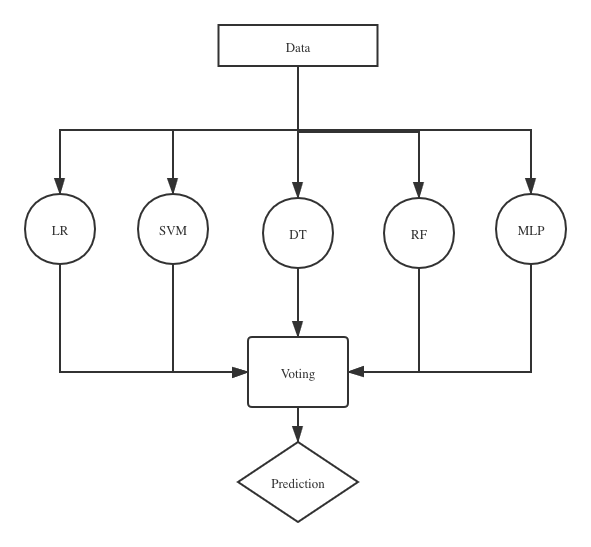
\includegraphics[width=0.5\textwidth]{image/voting}
	\caption{The voting classifier}
	\label{vcl}
\end{figure}


\subsubsection{Soft mode}
All the model prediction samples are the estimated value of the probability of certain categories, and the corresponding type with the highest probability is the final prediction result; This require that each model of the set can estimate the probability. We have to enable the probability output of SVM.

I applied elimination strategy to the model, that is, minimizing the weight of poor performed classifier and turn up the weight of well performed classifier. Here, I use the average f1-score if classifiers as the weight vector.

\section{Evaluation}
The dataset is divided into training and testing sets, train:test = 7:3.

The traditional F-measure or balanced F-score (F1 score) is the harmonic mean of precision and recall.
The number of positive sample is $P$, The number of negative sample is $N$

The recognition rate $Acc=\frac{TP+TN}{TP+TN+FP+FN}=\frac{TP+TN}{P+N}$

$\text{Recall}=\frac{TP}{TP+FN}=\frac{TP}{P}$

$\text{Precision}=\frac{TP}{TP+FP}$

$F_1=\frac{2 T P}{2 T P+F N+F P}=\frac{2 \cdot \text { Precision } \cdot \text { Recall}}{\text {Precision }+\text { Recall}}$

Recall reflects the classification model H's ability to identify positive samples. The higher the recall, the stronger the model's ability to identify positive samples. Precision reflects the model's ability to distinguish negative samples. The higher the precision, the better the model's discrimination of negative samples. The stronger the ability. F1-score is a combination of the two. The higher the F1-score, the more robust the classification model. 

\subsection*{Logistic Regression Classifier}
\begin{figure}[H]
	\centering
	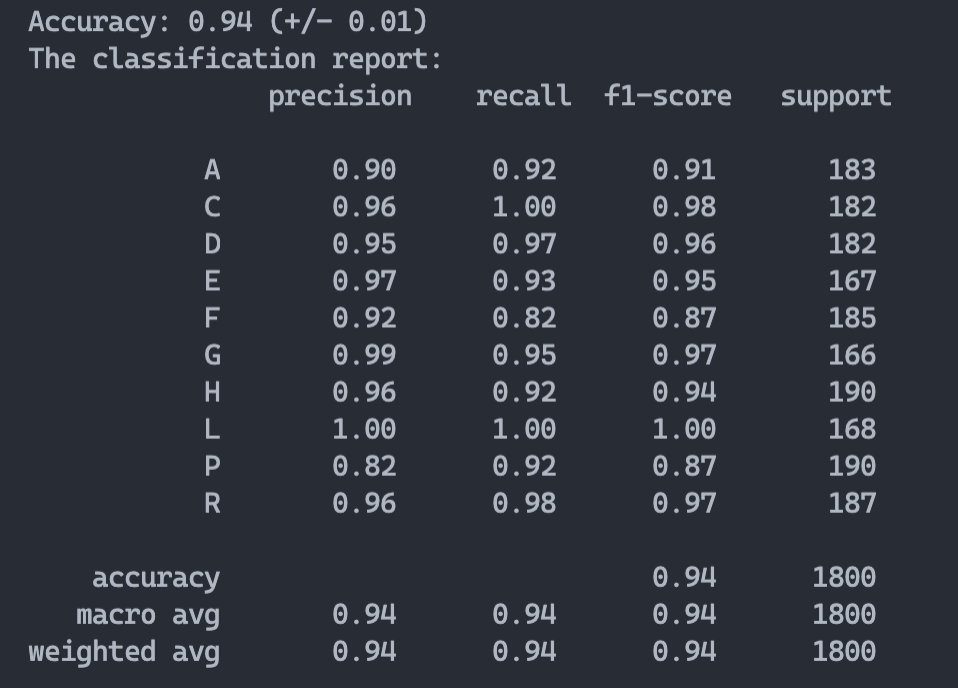
\includegraphics[width=0.4\textwidth]{image/lrpf}
	\caption{The LR performance}
	\label{lrpf}
\end{figure}

\subsection*{SVM}
\begin{figure}[H]
	\centering
	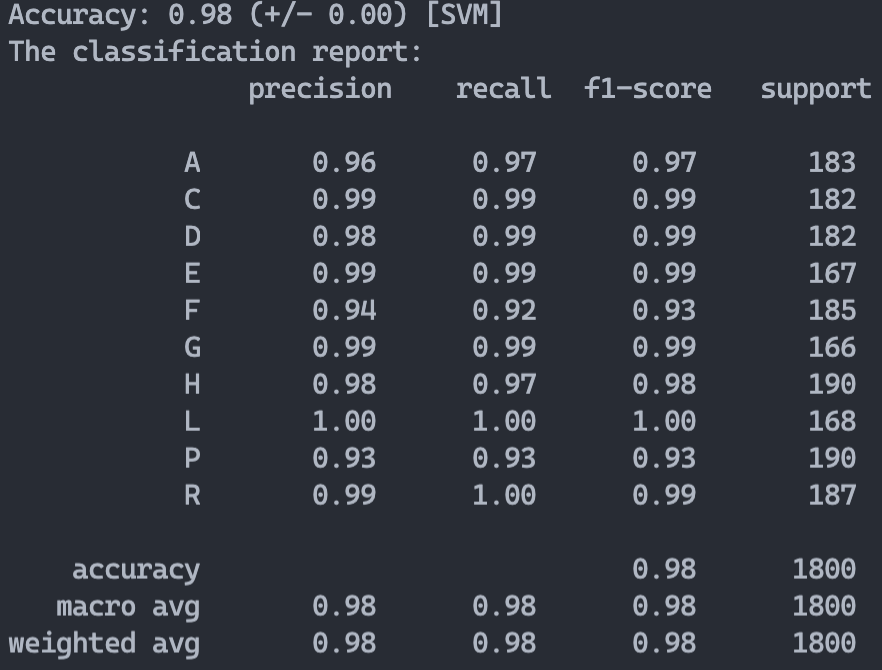
\includegraphics[width=0.4\textwidth]{image/svmpf}
	\caption{The SVM performance}
	\label{svmpf}
\end{figure}

\subsection*{SGD}
\begin{figure}[H]
	\centering
	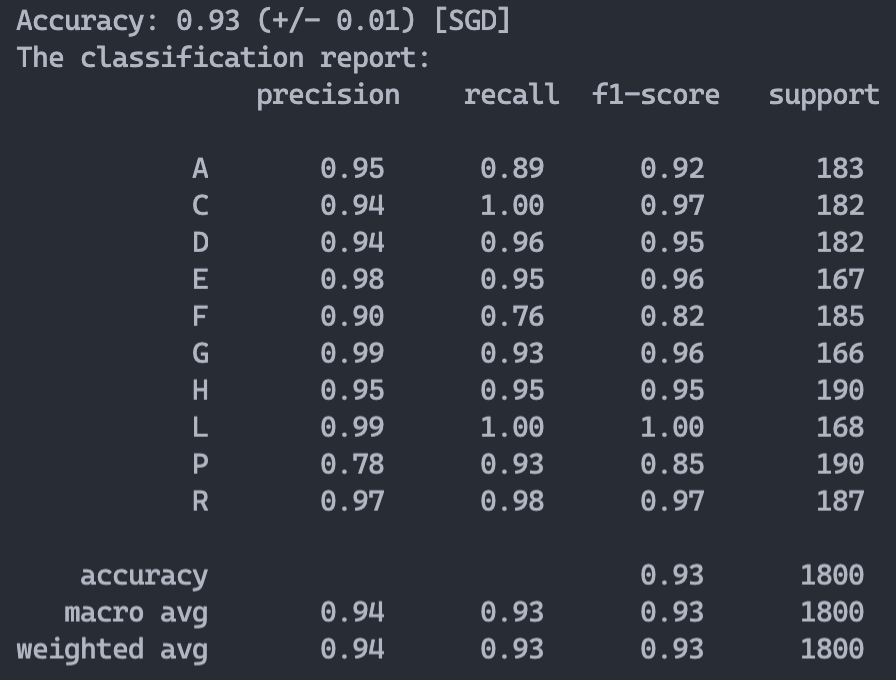
\includegraphics[width=0.4\textwidth]{image/sgdpf}
	\caption{The SGD performance}
	\label{sgdpf}
\end{figure}

\subsection*{Decision Tree}
\begin{figure}[H]
	\centering
	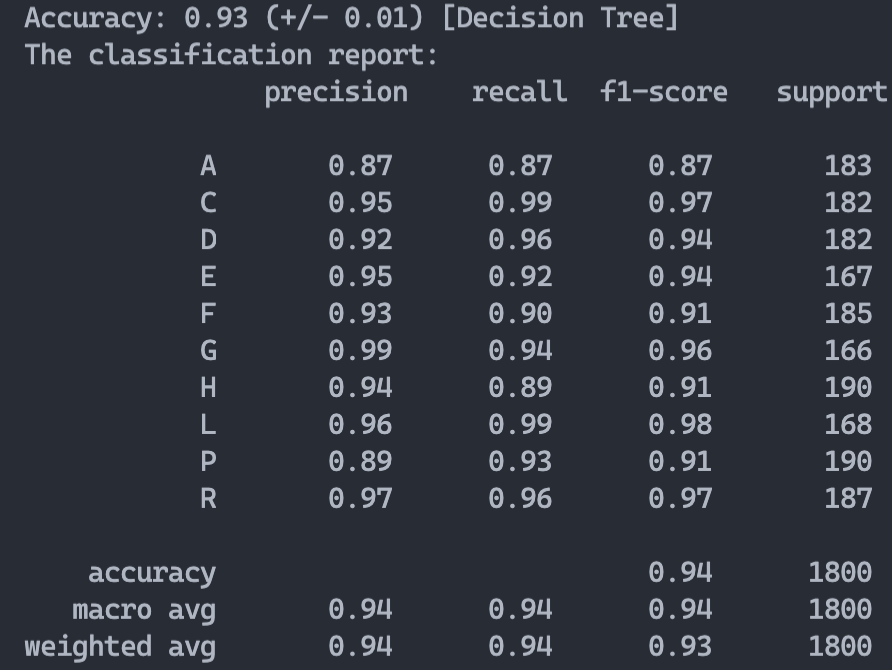
\includegraphics[width=0.4\textwidth]{image/dtpf}
	\caption{The Decision Tree performance}
	\label{dtpf}
\end{figure}

\subsection*{Random Forest}
\begin{figure}[H]
	\centering
	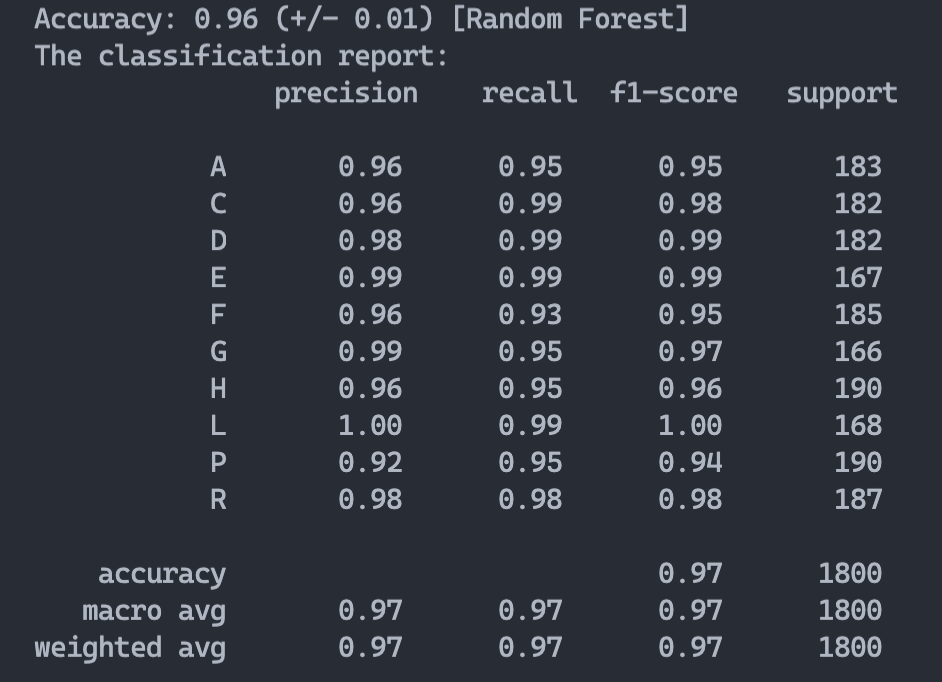
\includegraphics[width=0.4\textwidth]{image/rfpf}
	\caption{The Random Forest performance}
	\label{rfpf}
\end{figure}

\subsection*{Extratree}
\begin{figure}[H]
	\centering
	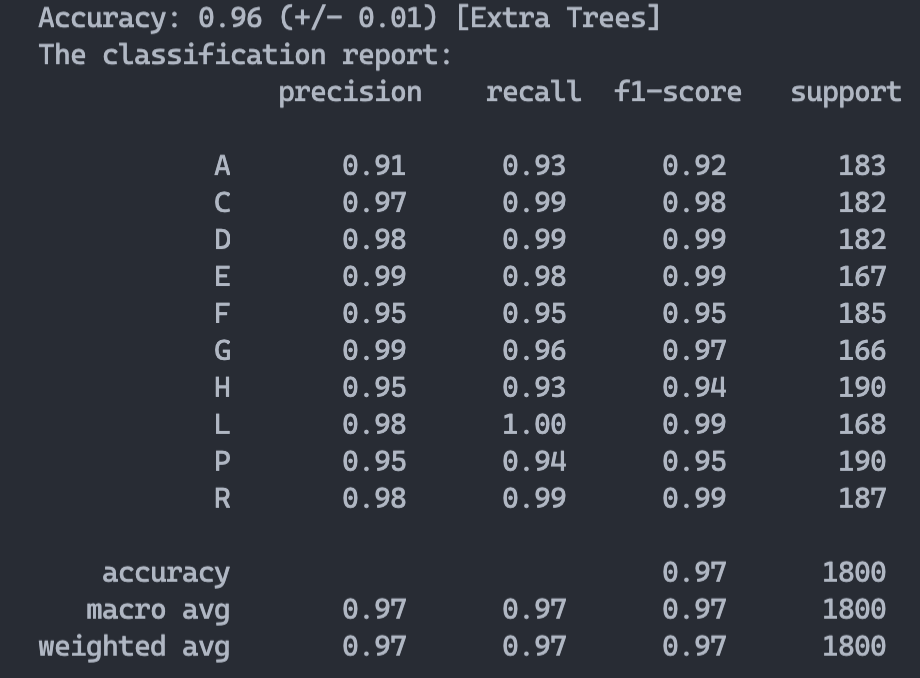
\includegraphics[width=0.4\textwidth]{image/etpf}
	\caption{The Extratree performance}
	\label{etpf}
\end{figure}


\subsection*{MLP}
\begin{figure}[H]
	\centering
	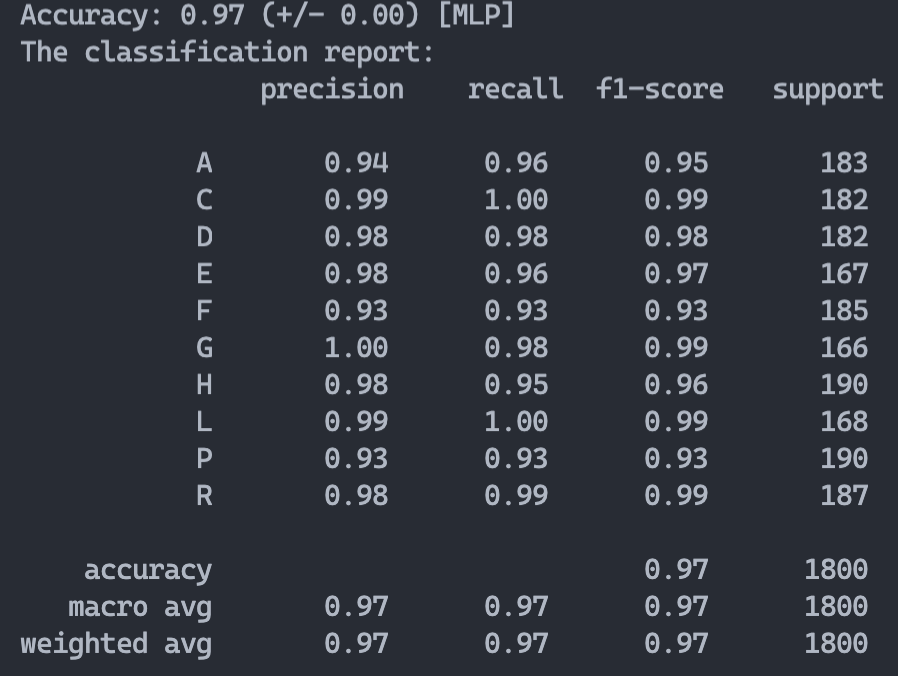
\includegraphics[width=0.4\textwidth]{image/mlppf}
	\caption{The MLP performance}
	\label{mlppf}
\end{figure}

\subsection*{Ensembling (Hard voting)}
\begin{figure}[H]
	\centering
	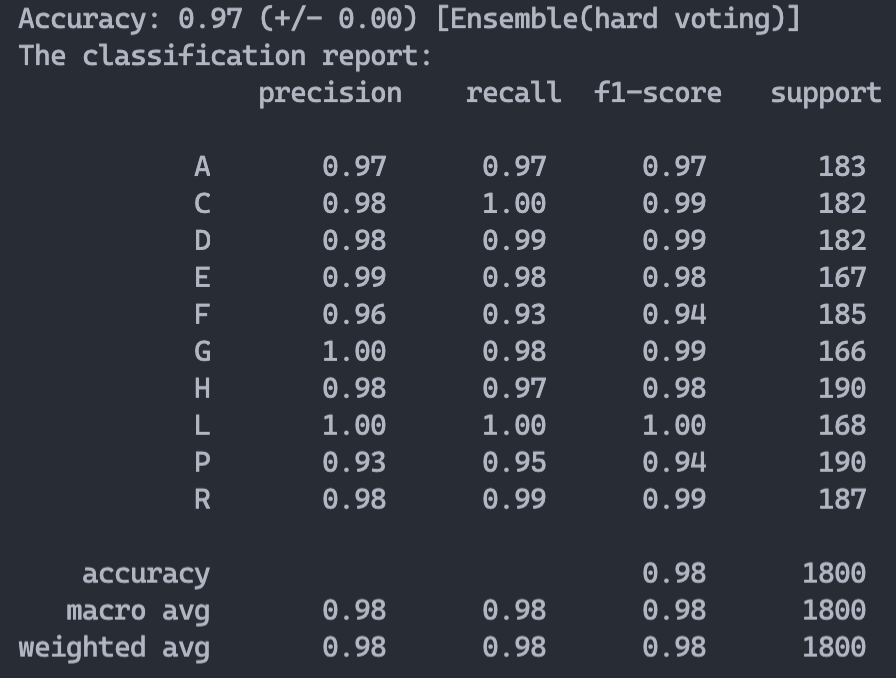
\includegraphics[width=0.4\textwidth]{image/hvpf}
	\caption{The Ensembling (Hard voting) performance}
	\label{hvpf}
\end{figure}

\subsection*{Ensembling (Soft voting)}
\begin{figure}[H]
	\centering
	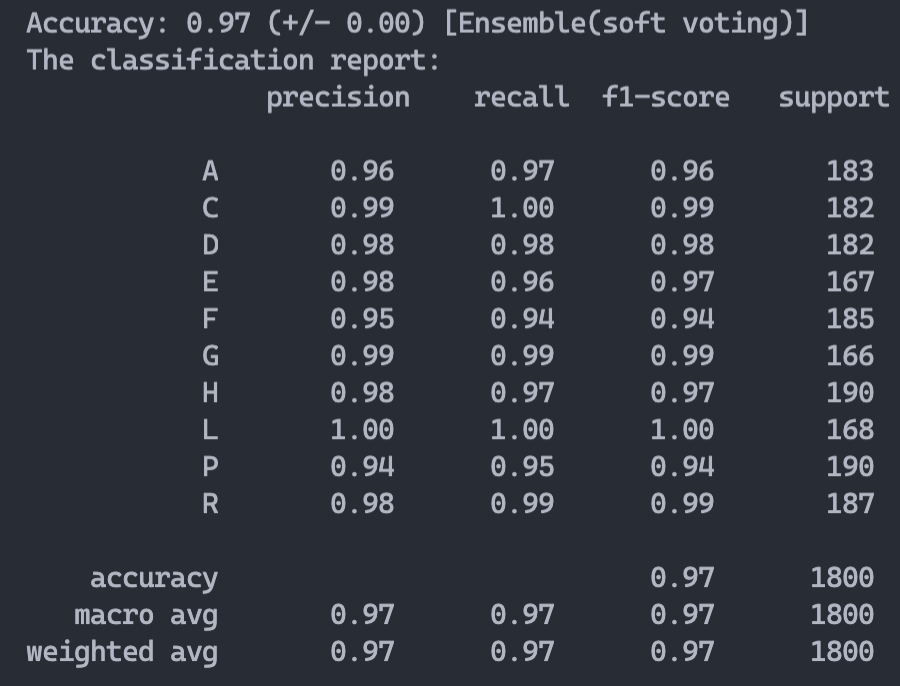
\includegraphics[width=0.4\textwidth]{image/svpf}
	\caption{The Ensembling (Soft voting) performance}
	\label{svpf}
\end{figure}

\subsection{Analysis}
Generally, The SVM and Hard voting Ensembling classifier have the best performance. Hard voting classifier perform better when precision/recall bias of each label is taken into concern. The Soft voting classifier, MLP and Random Forest also have ideal performance. The SGD, LR and Decision tree model is too simplified to perform well in this task. 

\section{Conclusion}
We showed the Ensembling can improve the performance of the classifiers, with which the classification can resist the disturbance of some noise. The voting ensembling is a kind of bagging, which mean that we can perform parallel learning in FPGA or GPU to accelerate the computing.


\bibliography{ref}
\end{document}
